\documentclass[10pt,letterpaper]{article}
\usepackage{tools}
\usepackage{enumitem}
%\settextfont{B Nazanin}
\usepackage{lipsum}
\setlength{\parskip}{3mm}
\setlength{\parindent}{0mm}
\newcommand{\wid}{0.49\textwidth}
\newcommand{\widone}{60mm}
\begin{document}
\Large
\begin{center}
In the name of beauty

7th problem set of ComNet course
\hl
\end{center}
Q1) 
\begin{enumerate}[label=\alph*-]
\item
False. The typical network-layer Internet service does not provide the order of packet arrival, jitter or even the eventual delivery of the packets at receiver.
\item
True. In contrast to the difference between connectionless and connection-oriented services in Transport Layer, at the Network Layer both the end systems and routers are involved.
\item
False. Routers need to also implement all the layers beneath layer 3, including layer 2.
\item
True. Also the data plane manages the routing process alongside the control plane.
\end{enumerate}

Q2) a. In the step of request, note that we might have more than one DHCP server present in the network and so we must address all of them.

In the step of ACK, we might have many users requesting for an IP address, so we still need to use a broadcast IP address.

b. (We choose the IP address of the web-server to be 10.20.30.40. The choice is arbitrary.)
\[
\begin{split}
&\text{From host to first-hop router:} 
\\&\text{src. IP Address = 172.17.1.39\quad,\quad src. port number = 10000}
\\&\text{dest. IP Address = 10.20.30.40\quad,\quad dest. port number = 80}
%\\&
\\&\text{From first-hop router to the web-server:} 
\\&\text{src. IP Address = 10.250.96.8\quad,\quad src. port number = 80}
\\&\text{dest. IP Address = 10.20.30.40\quad,\quad dest. port number = 80}
%%
\\&\text{From the web-server to the first-hop router:} 
\\&\text{src. IP Address = 10.20.30.40\quad,\quad src. port number = 80}
\\&\text{dest. IP Address = 10.250.96.8\quad,\quad dest. port number = 80}
%%%
\\&\text{From the first-hop router to the host:} 
\\&\text{src. IP Address = 10.20.30.40\quad,\quad src. port number = 80}
\\&\text{dest. IP Address = 172.17.1.39\quad,\quad dest. port number = 10000}
\end{split}
\]

Q3) We allocate $64=2^6$, $128=2^7$ and $16=2^4$ IP addresses to subnets 1,2 and 3 respectively. A possible assigned prefix is as follows:
$$
\text{Subnet 1 : }\{11011111.00000001.00010001\}.01******\implies223.1.17.64/26
$$
$$
\text{Subnet 2 : }\{11011111.00000001.00010001\}.1*******\implies223.1.17.128/25
$$
$$
\text{Subnet 3 : }\{11011111.00000001.00010001\}.0000****\implies223.1.17.0/28
$$

Q4) A queue of length $n$ has a probability of $p^n(1-p)$. Once a newly-arrived packet is arrived at the input of a queue with length of 5 or more, a dropping procedure is executed, so the desired probability becomes:
\[
\begin{split}
\Pr\{\text{Dropping the packet}\}&=
\sum_{n=5}^\infty
\Pr\{\text{Dropping the packet}|\text{Queue has length $n$}\}\\&\Pr\{\text{Queue has length $n$}\}
\\&=
{p^5+p^6+p^7\over 5}(1-p)+[p^8+p^9+p^{10}+\cdots](1-p)
\\&={p^5+4p^8\over 5}
\end{split}
\]
\newpage
Q5)

\begin{figure}[htbp]
\centering
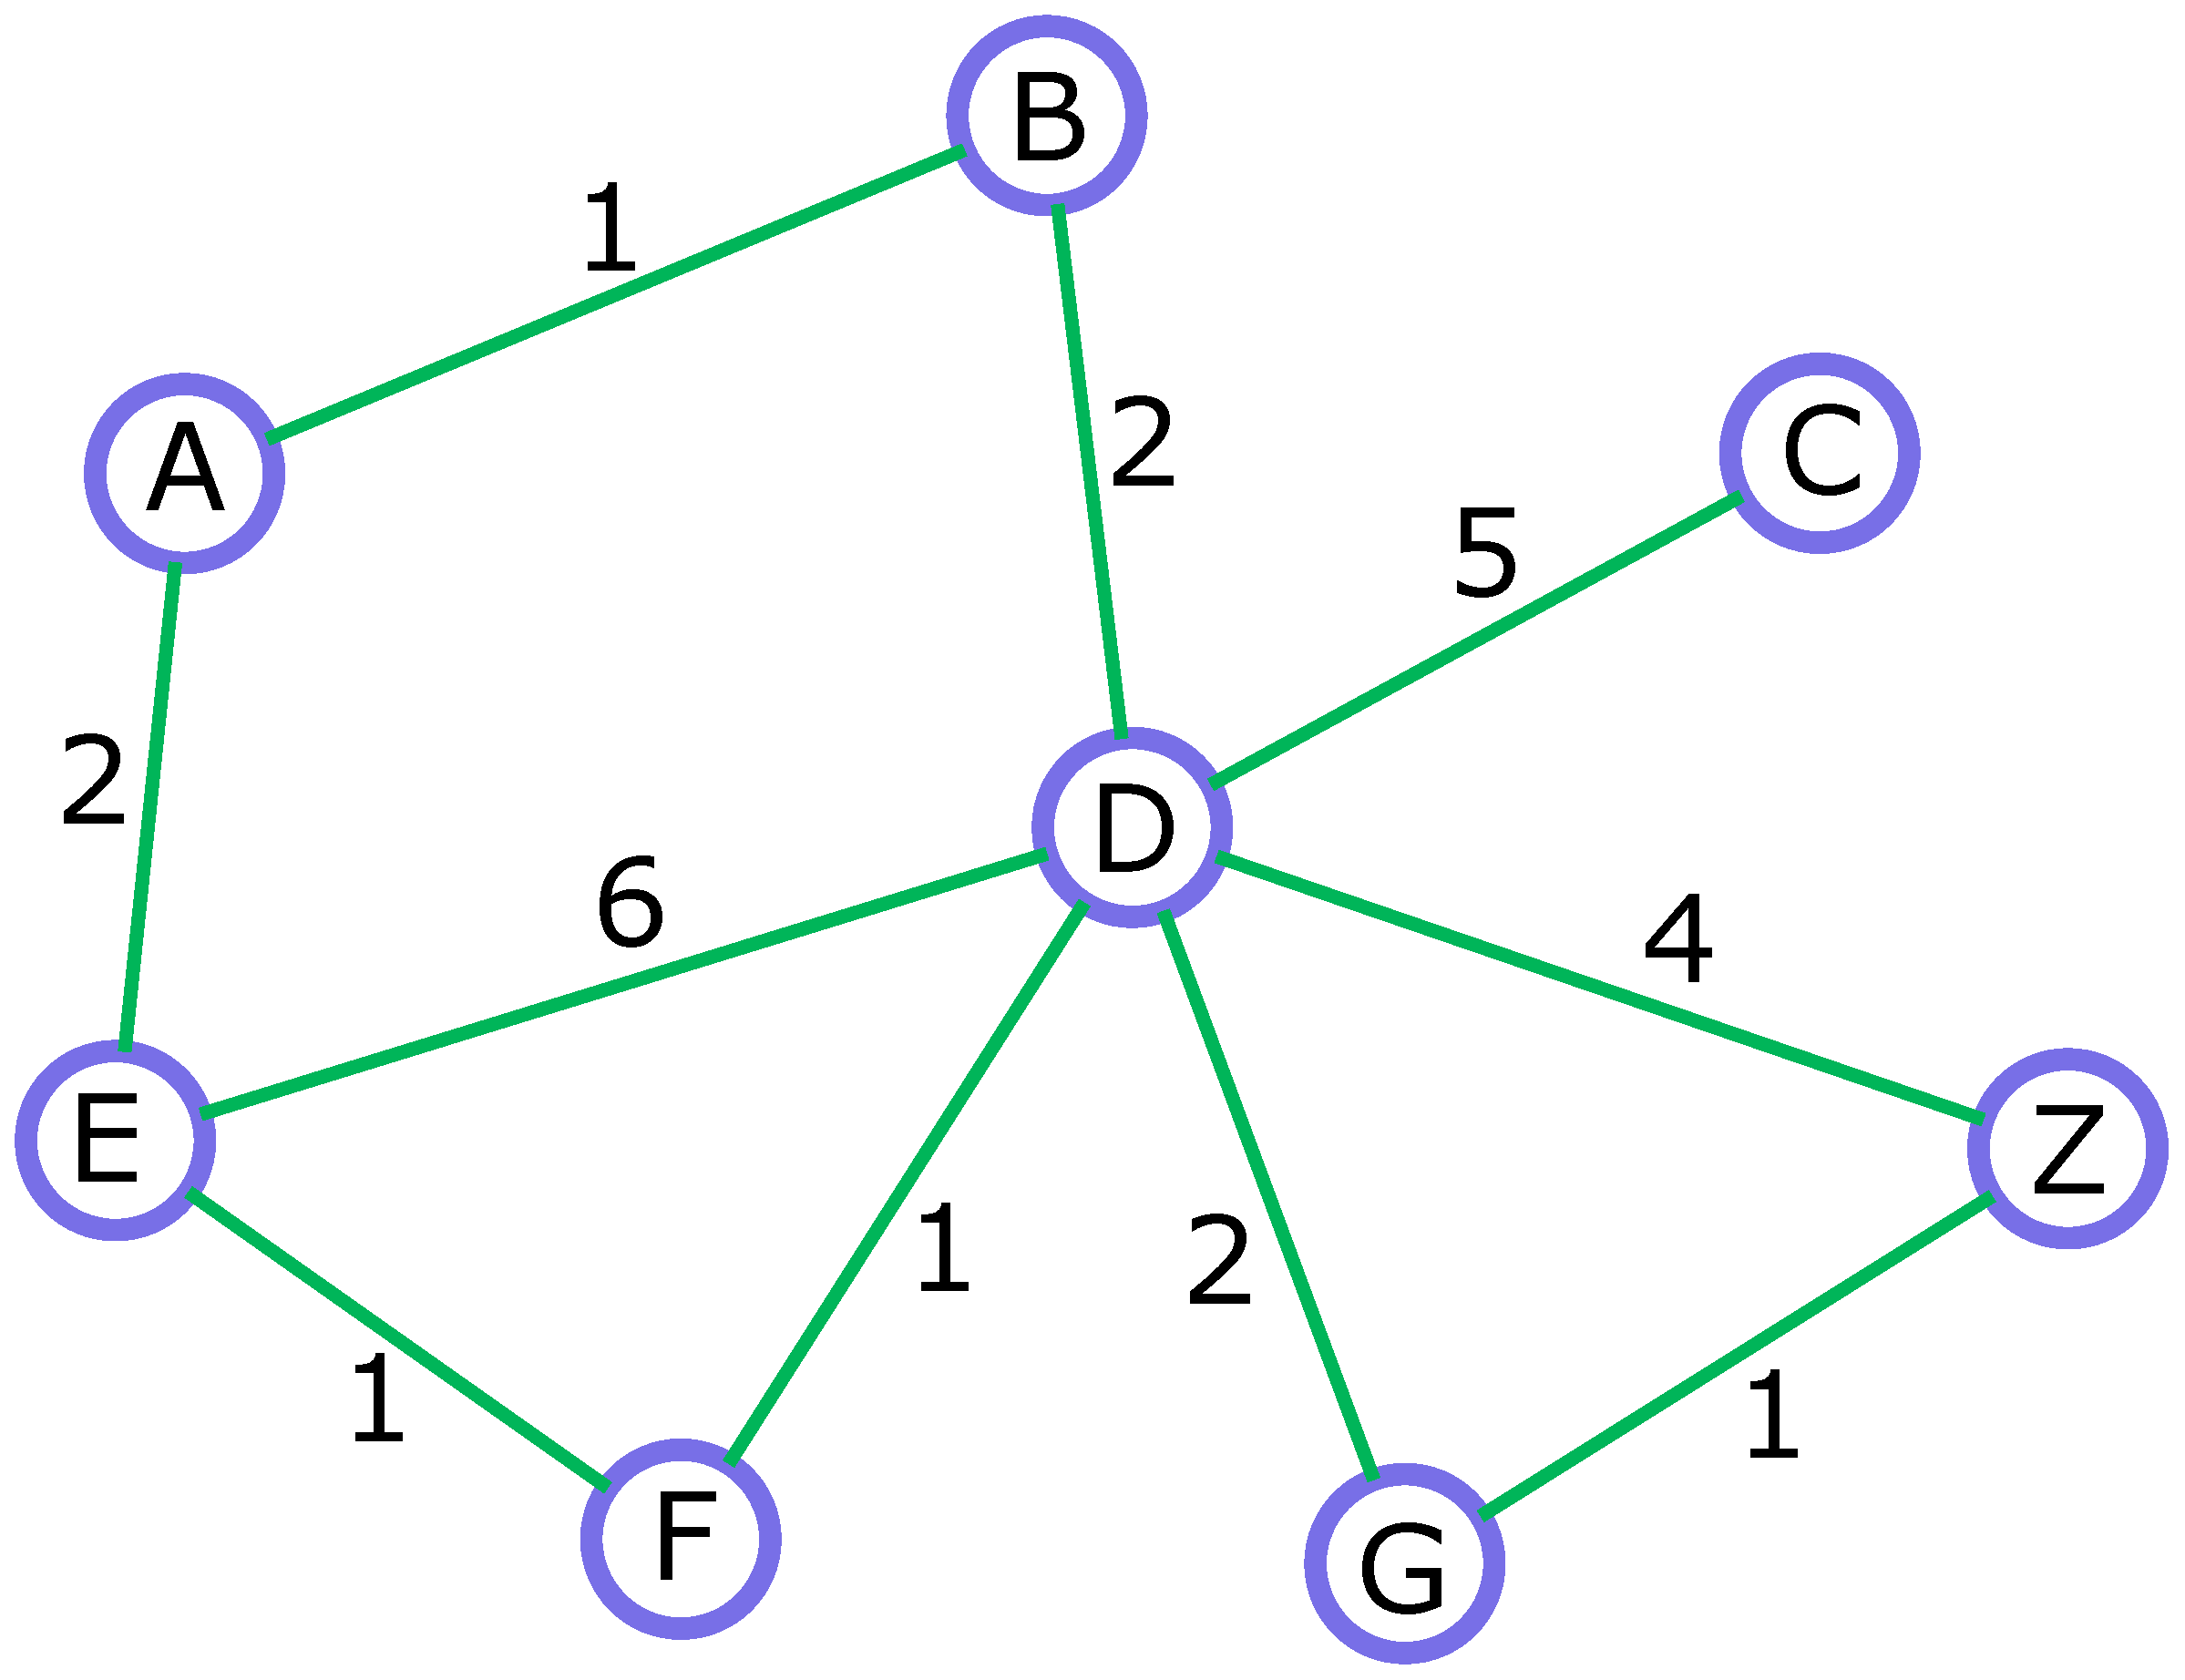
\includegraphics[width=100mm]{dij.eps}
\end{figure}
\begin{figure}[htbp]
\centering
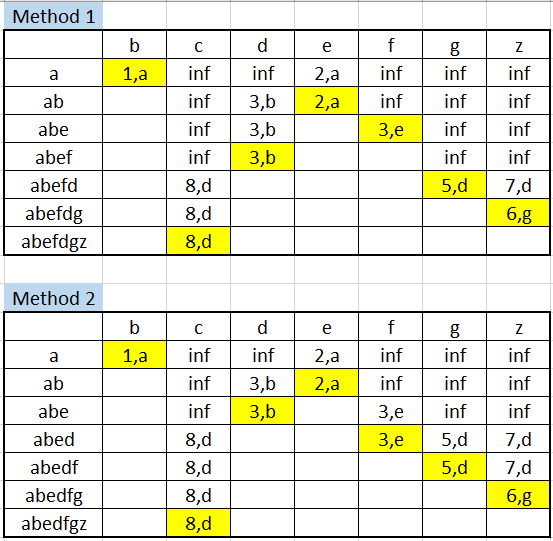
\includegraphics[width=100mm]{dij_tab.png}
\end{figure}
\end{document}